% !TEX program = xelatex
\documentclass[aspectratio=169,11pt]{beamer}

\usetheme{default}
\usecolortheme{default}
\setbeamertemplate{navigation symbols}{}
\setbeamertemplate{footline}[frame number]

\definecolor{frost}{RGB}{40,62,84}
\definecolor{ember}{RGB}{170,80,40}
\definecolor{stone}{RGB}{110,110,105}
\setbeamercolor{frametitle}{fg=frost}
\setbeamercolor{title}{fg=frost}
\setbeamercolor{structure}{fg=frost}
\setbeamercolor{alerted text}{fg=ember}

\usepackage{tikz}
\usetikzlibrary{positioning,arrows.meta}

%% Dragon alphabet (Pixel Sagas "Dovahkiin" font; requires XeLaTeX).
%% Letters map to single runes; digraph runes sit on accented capitals:
%% Ã=ah Ä=aa È=ei Ë=ey Î=ir Ï=ii Ö=oo Ù=ur Ü=uu
\usepackage{fontspec}
\newfontfamily\dragonfont{Dovahkiin.ttf}[Path=fonts/]
\newcommand{\dovah}[1]{{\dragonfont #1}}

%% Era title cards: a full-bleed screenshot with an in-game line over it.
%% Drop screenshots (ideally 16:9) into images/ as <name>.jpg or <name>.png;
%% until a file exists, a labelled placeholder is drawn instead.
%% Images are fitted (not cropped) into the area above the caption band, on black.
\newcommand{\shotimg}[1]{%
  \fill[black] (current page.south west) rectangle (current page.north east);
  \node[inner sep=0, anchor=north] at (current page.north)
    {\includegraphics[width=\paperwidth, height=\dimexpr\paperheight-3.2cm\relax, keepaspectratio]{#1}};
  \node[anchor=north east, font=\tiny, text=white, opacity=0.7] at ([xshift=-2pt, yshift=-2pt]current page.north east) {Image: UESP};}
\newcommand{\shotfill}[2]{%
  \IfFileExists{images/#1.jpg}{\shotimg{images/#1.jpg}}{%
  \IfFileExists{images/#1.png}{\shotimg{images/#1.png}}{%
  \fill[frost!15] (current page.south west) rectangle (current page.north east);
  \node[align=center, font=\small, text=stone] at ([yshift=1.4cm]current page.center)
    {\textbf{Screenshot:} #2\\[0.2em]{\scriptsize\ttfamily images/#1.jpg}};}}}
% #1 image, #2 what the screenshot shows, #3 era label, #4 the line, #5 who says it
\newcommand{\eracard}[5]{%
  \begin{frame}[plain]
    \begin{tikzpicture}[remember picture, overlay]
      \shotfill{#1}{#2}
      \fill[black, opacity=0.65] (current page.south west) rectangle ([yshift=3.2cm]current page.south east);
      \node[anchor=south west, text width=0.86\paperwidth, align=left, text=white]
        at ([xshift=0.9cm, yshift=0.45cm]current page.south west)
        {{\scriptsize\bfseries\color{ember!50!white}#3}\\[0.4em]
         {\large\itshape #4}\\[0.4em]
         {\small --- #5}};
    \end{tikzpicture}
  \end{frame}}
% Closing line on a history slide: where this past is still alive in 4E 201.
\newcommand{\stillhere}[1]{\par\vfill{\small\textbf{\color{ember}Still here in 4E 201:} #1}}

\title{Archaeogaming: A Site Visit to Skyrim}
\subtitle{MIT Splash 2026}
\author{Arnav Sood}
\date{\today}

\begin{document}

\begin{frame}
  \titlepage
  \begin{center}
    \textbf{``Skyrim's harshness has a way of carving a man down to his true self''}\\[0.3em]
    \small -- General Tullius (Imperial Legion)
  \end{center}
\end{frame}

\begin{frame}
  \begin{itemize}
    \item {\color<3->{stone}\textbf{``[Ysgramor] came from the ancient homeland and killed all the elves. But not all of them, because some of them are still here.''}}
    \item[] {\color<3->{stone}\begin{center} \small -- Farkas (Companion) \end{center}} \pause
    \item {\color<3->{stone}\textbf{``Everything's for sale, my friend. Everything. If I had a sister, I'd sell her in a second.''}}
    \item[] {\color<3->{stone}\begin{center} \small -- Belethor (Merchant) \end{center}} \pause
    \item \textbf{``Nivahriin muz fen siiv nid aaz het.'' {\color{red} Cowardly men will find no mercy here}}
    \item[] {\centering\large\dovah{NIVÃRÏN MUZ FEN SÏV NID ÄZ HET}\par}
    \item[] {\begin{center} \small -- Morokei (Dragon Priest, Undead) \end{center}}
  \end{itemize}
\end{frame}

% ------------------------------------------------------------------
\begin{frame}{Today's question}
  \Large
  Every ruin is a record of a conversation.\\[1em]
  \normalsize
  At each layer of the barrow, we'll ask:
  \begin{enumerate}
    \item \textbf{Who} built this, and \textbf{for whom}?
    \item \textbf{What} is it meant to convey, and how does the design show it?
    \item \textbf{What has happened} to it since?
  \end{enumerate}
  \vfill
  \small\color{stone}To date what we find, we first need a timeline.
\end{frame}

% ------------------------------------------------------------------
\begin{frame}{The calendar of Tamriel}
  \begin{center}
    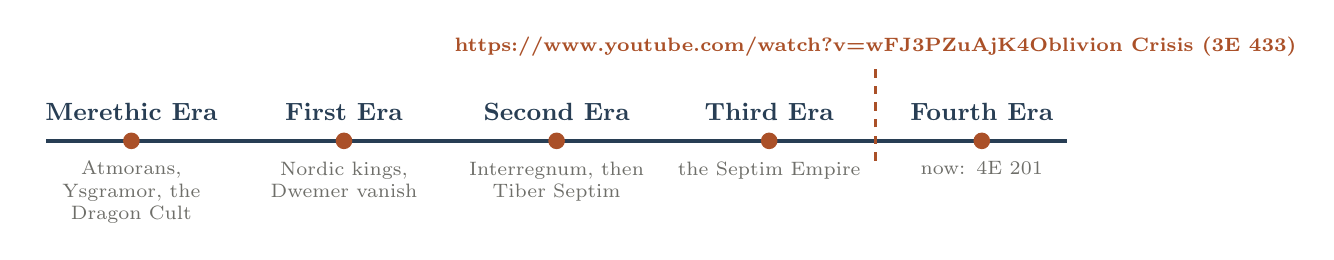
\begin{tikzpicture}[x=0.9cm,y=1cm]
      \draw[very thick, frost] (0,0) -- (14.4,0);
      \foreach \x/\lab/\sub in {
          1.2/Merethic Era/{Atmorans, Ysgramor, the Dragon Cult},
          4.2/First Era/{Nordic kings, Dwemer vanish},
          7.2/Second Era/{Interregnum, then Tiber Septim},
          10.2/Third Era/{the Septim Empire},
          13.2/Fourth Era/{now: 4E 201}}
        {
          \fill[ember] (\x,0) circle (3pt);
          \node[above=4pt, font=\small\bfseries, text=frost] at (\x,0) {\lab};
          \node[below=4pt, font=\scriptsize, text=stone, text width=2.4cm, align=center] at (\x,0) {\sub};
        }
      \draw[thick, dashed, ember] (11.7,-0.25) -- (11.7,0.95);
      \node[above, font=\scriptsize\bfseries, text=ember] at (11.7,0.95) {\href{https://www.youtube.com/watch?v=wFJ3PZuAjK4}{Oblivion Crisis (3E 433)}};
    \end{tikzpicture}
  \end{center}
  \vspace{1em}
  \begin{itemize}
    \item Dates are written like \alert{1E 700} = year 700 of the First Era.
    \item Eras reset at big turning points, so ``older'' is not just ``smaller number.''
          Merethic dates even count \emph{down}: \alert{ME 1000} is older than ME 1.
    \item In-game sources often \emph{disagree} about dates. So do real ones.
  \end{itemize}
  \vfill
  {\small\color{stone}Asked who wrote the Elder Scrolls, the College librarian replies:
    \emph{``It would take a month to explain to you how that very question doesn't even make sense.''}
    --- Urag gro-Shub}
\end{frame}

% ------------------------------------------------------------------
\eracard{saarthal}{the College's dig at Saarthal}{MERETHIC ERA \textperiodcentered{} c.\ ME 1000}
  {``Ysgramor was the hero who started the Companions. Wuuthrad was his weapon. He came from the ancient homeland and killed all the elves. But not all of them, because some of them are still here.''}
  {Farkas of the Companions, who still keep Ysgramor's tomb, 4E 201}

% ------------------------------------------------------------------
\begin{frame}{Merethic Era: the first footprints}
  \begin{columns}[T]
    \begin{column}{0.58\textwidth}
      \begin{itemize}
        \item<1-> {\color<2->{stone}Skyrim settled by the \textbf{elves} first: the Snow Elves (Falmer).}
        \item<2-> {\color<3->{stone}\textbf{c.\ ME 1000}: humans from \textbf{Atmora}, a frozen continent to the north, settle at \textbf{Saarthal}.}
        \item<3-> {\color<4->{stone}The elves destroy Saarthal: the \alert<3>{Night of Tears}.}
        \item<4-> {\color<5->{stone}\textbf{Ysgramor} returns with the \textbf{Five Hundred Companions} and reclaims Skyrim.}
        \item<5-> {\color<6->{stone}Nords inhabit the space for (at least) the next 4500 years.}
        \item<6-> {\color{red} Are the Nords now indigenous?}
      \end{itemize}
    \end{column}
    \begin{column}{0.38\textwidth}
      \small
      \textbf{Sites from this layer}\\[0.3em]
      \emph{Nord:} Saarthal\\
      Ysgramor's Tomb\\
      Yngol Barrow\\
      Windhelm: the Palace of the Kings\\
      Whiterun: Jorrvaskr \& the Skyforge\\[0.3em]
      \emph{Snow Elf:} the Forgotten Vale\\[1em]
      \color{stone} How much of a founding legend should we believe?
    \end{column}
  \end{columns}
\end{frame}

% ------------------------------------------------------------------
\eracard{dragon-priest}{Morokei, dragon priest of Labyrinthian}{MERETHIC ERA \textperiodcentered{} THE DRAGON CULT}
  {{\normalfont\dovah{NIVÃRÏN MUZ FEN SÏV NID ÄZ HET}}\\[0.2em]
   ``Nivahriin muz fen siiv nid aaz het.''\\[0.2em]
   {\normalsize\upshape Cowardly men will find no mercy here.}}
  {Morokei, dragon priest of Labyrinthian, still awake in 4E 201}

% ------------------------------------------------------------------
\begin{frame}{Merethic Era: the Dragon Cult}
  \begin{columns}[T]
    \begin{column}{0.58\textwidth}
      \begin{itemize}
        \item Before recorded history, \textbf{dragons} rule the Nords, and are worshipped as gods.
        \item \textbf{Dragon priests} rule in their name from \textbf{Bromjunaar}, behind masks of metal.
        \item The faithful dead go into \alert{barrows}, and rise as \textbf{draugr} to guard them.
        \item The dragons' words are cut into \textbf{Word Walls}. Read one, and you learn to Shout.
      \end{itemize}
    \end{column}
    \begin{column}{0.38\textwidth}
      \small
      \textbf{What to look for}\\[0.3em]
      Dragon imagery on arches\\
      Claw doors \& puzzle pillars\\
      Draugr in burial alcoves\\
      Word Walls at the deepest point\\[1em]
      \color{stone}\emph{This is the main layer we'll dig through today.}
    \end{column}
  \end{columns}
  \stillhere{the draugr are still on guard. Walk in, and they wake up.}
\end{frame}

% ------------------------------------------------------------------
\eracard{paarthurnax}{Paarthurnax on the summit of the Throat of the World}{THE DRAGON WAR \textperiodcentered{} LATE MERETHIC ERA}
  {``What is better --- to be born good, or to overcome your evil nature through great effort?''}
  {Paarthurnax, once Alduin's lieutenant, who switched sides and taught men to Shout}

% ------------------------------------------------------------------
\begin{frame}{The Dragon War: end of the Merethic Era}
  \begin{itemize}
    \item Late in the Merethic Era, the Nords rise against their dragon gods.
    \item A dragon, \textbf{Paarthurnax}, breaks ranks and teaches them the \textbf{Thu'um} (the Voice). Men learn to Shout back.
    \item \textbf{Alduin}, the World-Eater, cannot be killed. On the \textbf{Throat of the World}, heroes use an Elder Scroll to cast him out of time.
    \item The Dragon Cult does not vanish overnight: holdouts survive \emph{into the First Era}. \alert{Forelhost} falls only c.\ \textbf{1E 140}.
  \end{itemize}
  \vfill
  \begin{block}{Why this matters for a barrow}
    The tombs we explore were built by a religion that \emph{lost}. Who keeps a tomb going when its builders' world is gone?
  \end{block}
  \stillhere{Paarthurnax still sits on the summit. And Alduin's exile is running out.}
\end{frame}

% ------------------------------------------------------------------
\eracard{high-hrothgar}{High Hrothgar, home of the Greybeards}{FIRST ERA \textperiodcentered{} 1E 1 -- 1E 2920}
  {``Dovahkiin!'' \quad {\normalfont\dovah{DOVÃKÏN}}}
  {the Greybeards, keepers of Jurgen Windcaller's Way of the Voice, Shouting from High Hrothgar so all Skyrim hears}

% ------------------------------------------------------------------
\begin{frame}{First Era: kings, elves, and dwarves}
  \begin{itemize}
    \item \textbf{1E 143}: \textbf{King Harald}, the first historical king of the Nords, unites Skyrim. His successors push its borders into Cyrodiil, Morrowind, and High Rock.
    \item The \textbf{Dwemer} (``dwarves,'' really elves) build vast underground cities, and enslave and blind the Snow Elves, who become today's \textbf{Falmer}.
    \item \alert{1E 700}: Battle of Red Mountain. The Dwemer \emph{disappear}, all of them, all at once.
    \item \textbf{Jurgen Windcaller} survives defeat there and founds the \textbf{Way of the Voice}: the Thu'um is for meditation, not war. His followers become the \textbf{Greybeards}.
  \end{itemize}
  \vfill
  {\small\color{stone}Dwemer ruins are a whole other class. Today: Nords only.}
  \stillhere{the Greybeards still meditate on High Hrothgar, and the Falmer still hunt in the dark below.}
\end{frame}

% ------------------------------------------------------------------
\eracard{talos-shrine}{Heimskr preaching at the statue of Talos in Whiterun}{SECOND \& THIRD ERAS \textperiodcentered{} THE SEPTIM EMPIRE}
  {``Talos the Mighty! Talos the Unerring! Talos the Unassailable!''}
  {Heimskr, preaching in Whiterun's square, 4E 201, to the Nord who became a god --- and whom the Empire has now banned}

% ------------------------------------------------------------------
\begin{frame}{Second and Third Eras: Skyrim inside an empire}
  \begin{itemize}
    \item After the fractured \textbf{Interregnum} (from 2E 430), \textbf{Tiber Septim} (a Nord, by some accounts) unites Tamriel in \textbf{2E 896}; the Third Era starts the next year.
    \item Legend says the Greybeards recognized him by his Thu'um, a link back to the dragon past.
    \item The \textbf{Septim Empire} lasts the whole Third Era. Its coin, the \alert{septim}, ends up everywhere.
    \item \textbf{3E 433}: the Oblivion Crisis ends the Septim line. The Fourth Era begins.
  \end{itemize}
  \vfill
  \begin{block}{Remember the coin}
    Septims did not exist before this empire. If one is lying in a tomb, someone put it there \emph{later}.
  \end{block}
  \stillhere{septims in every purse, and Talos worshipped in secret.}
\end{frame}

% ------------------------------------------------------------------
\eracard{stormcloak-battle}{Stormcloaks storming Solitude}{FOURTH ERA \textperiodcentered{} 4E 201}
  {``My ancestors are smiling at me, Imperial. Can you say the same?''}
  {a Stormcloak soldier, mid-battle, in a civil war fought over the past}

% ------------------------------------------------------------------
\begin{frame}{Fourth Era: the still-sodden battlefields}
  \begin{columns}[T]
    \begin{column}{0.55\textwidth}
      \begin{itemize}
        \item \textbf{4E 5}: Red Mountain erupts (the Red Year).
        \item \textbf{4E 171--175}: the \textbf{Great War} with the elven Aldmeri Dominion.
        \item The peace treaty (the \textbf{White-Gold Concordat}) \alert{bans worship of Talos}, the god Tiber Septim became.
        \item \textbf{4E 201}: Ulfric Stormcloak kills the High King with his Voice. Civil war.
        \item And the dragons come back.
      \end{itemize}
    \end{column}
    \begin{column}{0.41\textwidth}
      \small
      \textbf{Imperials}\\
      Keep the Empire together; accept the treaty.\\[0.6em]
      \textbf{Stormcloaks}\\
      Skyrim for the Nords; restore Talos.\\[1em]
      \color{stone}\emph{Both sides raid ancient tombs for symbols of legitimacy. (See: the Jagged Crown.)}
    \end{column}
  \end{columns}
\end{frame}

% ------------------------------------------------------------------
\begin{frame}{4,000 years, stacked}
  \begin{center}
    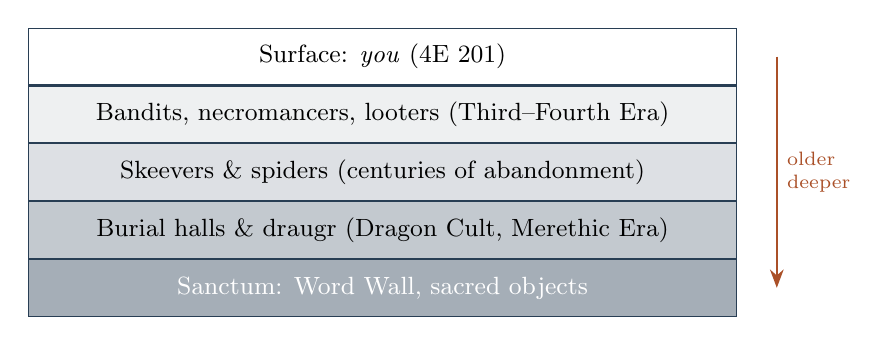
\begin{tikzpicture}[
        layer/.style={draw=frost, minimum width=9cm, minimum height=0.72cm, font=\small, align=center},
      ]
      \node[layer, fill=white]            (l0) {Surface: \emph{you} (4E 201)};
      \node[layer, fill=frost!8,  below=0pt of l0] (l1) {Bandits, necromancers, looters (Third--Fourth Era)};
      \node[layer, fill=frost!16, below=0pt of l1] (l2) {Skeevers \& spiders (centuries of abandonment)};
      \node[layer, fill=frost!28, below=0pt of l2] (l3) {Burial halls \& draugr (Dragon Cult, Merethic Era)};
      \node[layer, fill=frost!42, below=0pt of l3, text=white] (l4) {Sanctum: Word Wall, sacred objects};
      \draw[-{Stealth}, thick, ember] ([xshift=0.5cm]l0.east) -- node[right, font=\scriptsize, text=ember, align=left]{older\\deeper} ([xshift=0.5cm]l4.east);
    \end{tikzpicture}
  \end{center}
  \vspace{0.5em}
  \centering\small A barrow is a history book read from the back cover.
\end{frame}

% ------------------------------------------------------------------
\begin{frame}{The archaeologist's toolkit}
  \begin{description}[Terminus post quem]
    \item[Superposition] Lower layers are usually older than the ones above them.
    \item[Terminus post quem] A layer is no older than the newest object in it.\\
          {\small\color{stone}(A septim on the floor means ``Third Era or later.'')}
    \item[Reuse] Later people move into old places for new reasons.
    \item[Disturbance] Animals, looters, and visitors mix the layers up.
    \item[Provenance] Where has this object been since it was made?
    \item[Text vs.\ object] Inscriptions and journals can inform, or lie.
  \end{description}
\end{frame}

% ------------------------------------------------------------------
\begin{frame}{Let's dig}
  \centering
  \Huge Bleak Falls Barrow\\[0.6em]
  \normalsize\color{stone}On the mountain above Riverwood\\[2em]
  \color{black}
  \begin{tabular}{l}
    1. \textbf{Who} built this, and \textbf{for whom}? \\[0.3em]
    2. \textbf{What} is it meant to convey?            \\[0.3em]
    3. \textbf{What has happened} to it since?
  \end{tabular}
\end{frame}

\end{document}
